% =============================================================================
% mahi-gpu (ASIC) -- Datasheet and Architecture Reference Manual
% Every number in this document is taken from the RTL / reports of repository
% commit dadec7f (see Appendix B for provenance).  Build:  make datasheet
% NOTE: the 'bytefield' package is not installed on the build machine, so the
% instruction bit-field diagrams use a small TikZ macro (\bitfield) instead.
% =============================================================================
\documentclass[10pt,a4paper]{report}
\usepackage[T1]{fontenc}
\usepackage{lmodern}
\usepackage[a4paper,margin=0.75in]{geometry}
\usepackage[table]{xcolor}
\usepackage{booktabs,longtable,array,tabularx,multirow}
\usepackage{tikz}
\usetikzlibrary{arrows.meta,positioning,shapes.geometric,fit,calc,backgrounds}
\usepackage{listings}
\usepackage{amsmath,amssymb}
\usepackage{microtype}
\usepackage{enumitem}
\usepackage{fancyhdr}
\usepackage{titlesec}
\usepackage[skins]{tcolorbox}
\usepackage[colorlinks=true,linkcolor=navy,urlcolor=navy,citecolor=navy]{hyperref}

% ---------------------------------------------------------------- colours
\definecolor{navy}{RGB}{0,32,96}
\definecolor{steel}{RGB}{70,110,160}
\definecolor{rowgray}{gray}{0.94}
\definecolor{hdrgray}{gray}{0.86}
\definecolor{warnred}{RGB}{160,30,30}
\definecolor{okgreen}{RGB}{30,110,50}
\definecolor{amber}{RGB}{190,120,0}

% ---------------------------------------------------------------- headings
\titleformat{\chapter}[display]{\sffamily\bfseries\color{navy}}{\large\chaptertitlename\ \thechapter}{4pt}{\Huge}
\titlespacing*{\chapter}{0pt}{-10pt}{18pt}
\titleformat{\section}{\sffamily\bfseries\Large\color{navy}}{\thesection}{0.6em}{}
\titleformat{\subsection}{\sffamily\bfseries\large\color{steel}}{\thesubsection}{0.6em}{}
\titleformat{\subsubsection}{\sffamily\bfseries\normalsize\color{steel}}{\thesubsubsection}{0.6em}{}
\pagestyle{fancy}\fancyhf{}
\fancyhead[L]{\sffamily\small\color{navy}mahi-gpu ASIC Datasheet}
\fancyhead[R]{\sffamily\small\color{navy}Rev 1.0 (preliminary)}
\fancyfoot[C]{\sffamily\small\thepage}
\renewcommand{\headrulewidth}{0.4pt}
\setlength{\parindent}{0pt}\setlength{\parskip}{4pt}
\renewcommand{\arraystretch}{1.15}
\setcounter{tocdepth}{2}

% ---------------------------------------------------------------- helpers
\newcommand{\sig}[1]{\texttt{\detokenize{#1}}}
\newcommand{\ins}[1]{\texttt{\detokenize{#1}}}
\newcommand{\reg}[1]{\texttt{R#1}}
\newcommand{\rowcol}{\rowcolors{2}{rowgray}{white}}
\newcommand{\tblhead}[1]{\cellcolor{hdrgray}\sffamily\bfseries #1}
\newtcolorbox{notebox}[2][]{enhanced,colback=blue!4,colframe=steel,fonttitle=\sffamily\bfseries,title={#2},boxrule=0.6pt,arc=2pt,#1}
\newtcolorbox{warnbox}[2][]{enhanced,colback=red!5,colframe=warnred,fonttitle=\sffamily\bfseries,title={#2},boxrule=0.6pt,arc=2pt,#1}
\newtcolorbox{statbox}[2][]{enhanced,colback=amber!8,colframe=amber,fonttitle=\sffamily\bfseries,title={#2},boxrule=0.6pt,arc=2pt,#1}

\lstdefinestyle{asm}{basicstyle=\ttfamily\footnotesize,commentstyle=\color{okgreen}\itshape,keywordstyle=\color{navy}\bfseries,
  frame=single,framerule=0.3pt,rulecolor=\color{steel},backgroundcolor=\color{rowgray},xleftmargin=2pt,xrightmargin=2pt,
  columns=fullflexible,keepspaces=true,showstringspaces=false,morecomment=[l]{;},
  morekeywords={ADD,SUB,MUL,DIV,MOD,AND,OR,XOR,SHL,SHR,MIN,MAX,ABS,NEG,MAC,POPCNT,CLZ,BREV,LUI,CONST,LDR,STR,LDSH,STSH,
  ATOM_ADD,ATOM_CAS,CMP,BRnzp,BRn,BRz,BRp,BRnz,BRnp,BRzp,CALL,RET_FN,SYNC,EXIT,FADD,FSUB,FMUL,FMA,NOP}}
\lstdefinestyle{rtl}{basicstyle=\ttfamily\footnotesize,frame=single,framerule=0.3pt,rulecolor=\color{steel},backgroundcolor=\color{rowgray},columns=fullflexible}

% Bit-field diagram: \bitfield{ width/hi/lo/label/fillcolour , ... }  (MSB first, 32 bits total)
\newcommand{\bitfield}[1]{%
 \par\smallskip\noindent\begin{tikzpicture}[x=0.455cm,y=0.78cm]
  \def\bfx{0}
  \foreach \bw/\bhi/\blo/\blab/\bcol in {#1} {
     \pgfmathparse{\bfx+\bw}\xdef\bfxn{\pgfmathresult}
     \draw[fill=\bcol!22,draw=navy,line width=0.5pt] (\bfx,0) rectangle (\bfxn,1);
     \node[font=\tiny\sffamily,text=navy,anchor=south west,inner sep=1pt] at (\bfx,1) {\bhi};
     \ifnum\bw>1\node[font=\tiny\sffamily,text=navy,anchor=south east,inner sep=1pt] at (\bfxn,1) {\blo};\fi
     \node[font=\scriptsize\sffamily,align=center] at ({(\bfx+\bfxn)/2},0.5) {\blab};
     \xdef\bfx{\bfxn}
  }
 \end{tikzpicture}\par\smallskip}

\begin{document}
\pagenumbering{roman}
% =============================================================================
% TITLE PAGE
% =============================================================================
\begin{titlepage}
\thispagestyle{empty}
\begin{tikzpicture}[remember picture,overlay]
  \fill[navy] (current page.north west) rectangle ([yshift=-7.2cm]current page.north east);
\end{tikzpicture}
\vspace*{1.2cm}
{\color{white}\sffamily\bfseries\fontsize{40}{44}\selectfont mahi-gpu\par}
\vspace{0.3cm}
{\color{white}\sffamily\Large 8-thread SIMT GPGPU core for SkyWater sky130\par}
\vspace{0.3cm}
{\color{white}\sffamily\large Datasheet and Architecture Reference Manual\par}
\vspace{4.3cm}
\begin{tabular}{@{}ll@{}}
\sffamily\bfseries Document revision & v1.0 --- \textbf{preliminary}\\
\sffamily\bfseries Date & 2026-10-21\\
\sffamily\bfseries Design source & repository commit \texttt{dadec7f}, directory \texttt{ASIC/src/rtl}\\
\sffamily\bfseries Top module & \texttt{gpu\_asic\_top}\\
\sffamily\bfseries Target process & SkyWater sky130A, \texttt{sky130\_fd\_sc\_hd}\\
\end{tabular}
\vfill
\begin{statbox}{Status of this document}
This manual describes the RTL \emph{as implemented}. It deliberately states what is \textbf{not} yet true of the chip:
the top level has no program/data memory attached, the physical-design run on record is incomplete and was made on an
almost-empty netlist, and barriers are only correct under warp-uniform control flow. See Chapter~\ref{ch:errata} (Errata)
before relying on any number in Chapter~\ref{ch:phys}.
\end{statbox}
\end{titlepage}

\tableofcontents
\clearpage
\pagenumbering{arabic}

% =============================================================================
\chapter{Overview}\label{ch:overview}
% =============================================================================
\section{Executive summary}
\textbf{mahi-gpu} is a compact general-purpose GPU core built around the SIMT execution model. One \emph{core} runs
\textbf{2 warps} of \textbf{4 lanes} each (8 hardware threads); every lane has its own integer ALU, single-precision FMA
unit, 32-entry register file, program counter and return stack. Warps are interleaved by a round-robin scheduler on a
classic five-stage in-order pipeline (IF, ID, EX, MEM, WB). A 5-stage pipelined IEEE-754-style FMA unit executes
\ins{FADD}, \ins{FSUB}, \ins{FMUL} and \ins{FMA} under a per-warp register scoreboard.
Memory is reached through a banked shared memory, an instruction cache, a 2-way write-through L1 data cache, and a
4-way write-back L2 cache with sector dirty bits and a victim write buffer. The host controls the device through a
32-bit Wishbone slave.

The ASIC build (\texttt{-DTARGET\_ASIC}) is a size-reduced profile of a configurable design that also targets FPGA and
simulation; all sizes in this manual are for the ASIC profile unless stated otherwise.

\section{Key characteristics}
\rowcol
\begin{longtable}{>{\raggedright\arraybackslash}p{5.2cm}>{\raggedright\arraybackslash}p{11.4cm}}
\tblhead{Characteristic} & \tblhead{Value}\\\endhead
Process / library & SkyWater sky130A, \texttt{sky130\_fd\_sc\_hd} (high density), 1.8\,V nominal\\
Supply corners analysed & 1.60\,V/100\,\textdegree C (ss), 1.80\,V/25\,\textdegree C (tt), 1.95\,V/$-$40\,\textdegree C (ff)\\
Flow & Yosys (via sv2v) $\rightarrow$ OpenROAD (floorplan, place, CTS, route) $\rightarrow$ Magic/KLayout, driven by LibreLane (\S\ref{sec:flow})\\
Clock constraint (target) & 25\,MHz (40\,ns period), single clock \sig{clk}, synchronous reset \sig{reset}\\
Cores / warps / lanes & 1 core / 2 warps / 4 lanes = \textbf{8 threads}\\
Pipeline & 5-stage in-order (IF, ID, EX, MEM, WB); FPU: 5-stage, fixed latency\\
Register file & 32 $\times$ 32-bit per thread; \reg{0}--\reg{28} general, \reg{29}--\reg{31} read-only\\
Instruction word & 32 bit, fixed width; 37 opcodes defined (0--36)\\
Program memory & 4\,K words (12-bit word address), external, 128-bit block interface\\
Global data memory & 16\,K words (14-bit word address), external, 128-bit block interface\\
Shared memory & \textbf{64 words} (256\,B), 4 banks $\times$ 16 words\\
L1 I-cache / L1 D-cache & 16 lines each; 16-byte lines (4 words); I: direct-mapped, D: 2-way, write-through\\
L2 cache & 64 lines (16 sets $\times$ 4 ways), 16-byte lines, 4 sectors/line with dirty bits, PLRU, write-back; 4-entry victim write buffer\\
Host interface & 32-bit Wishbone slave, single-cycle ack; \textbf{107 signal pins} (excl.\ power)\\
Synthesised logic area (pre-PnR) & 38\,657\,\textmu m\textsuperscript{2} / 3\,162 cells --- \textbf{not representative} (\S\ref{sec:flow})\\
Die size (floorplan) & 2.5\,mm $\times$ 2.5\,mm (6.25\,mm\textsuperscript{2}), absolute sizing\\
\end{longtable}

\section{Conventions}
Numbers: \texttt{0x} prefix hexadecimal. Bit ranges \texttt{[hi:lo]} are inclusive. Addresses in the memory system are
\emph{word} addresses unless stated. ``Lane'' and ``thread'' are used interchangeably within a warp.
Source citations use the form \texttt{file.sv:line} relative to \texttt{ASIC/src/rtl}.
The words \emph{limitation} and \emph{erratum} refer to the register in Chapter~\ref{ch:errata} (IDs \textbf{L1--L14}).

% =============================================================================
\chapter{System architecture and memory map}\label{ch:system}
% =============================================================================
\section{Block diagram}
\begin{figure}[ht]\centering
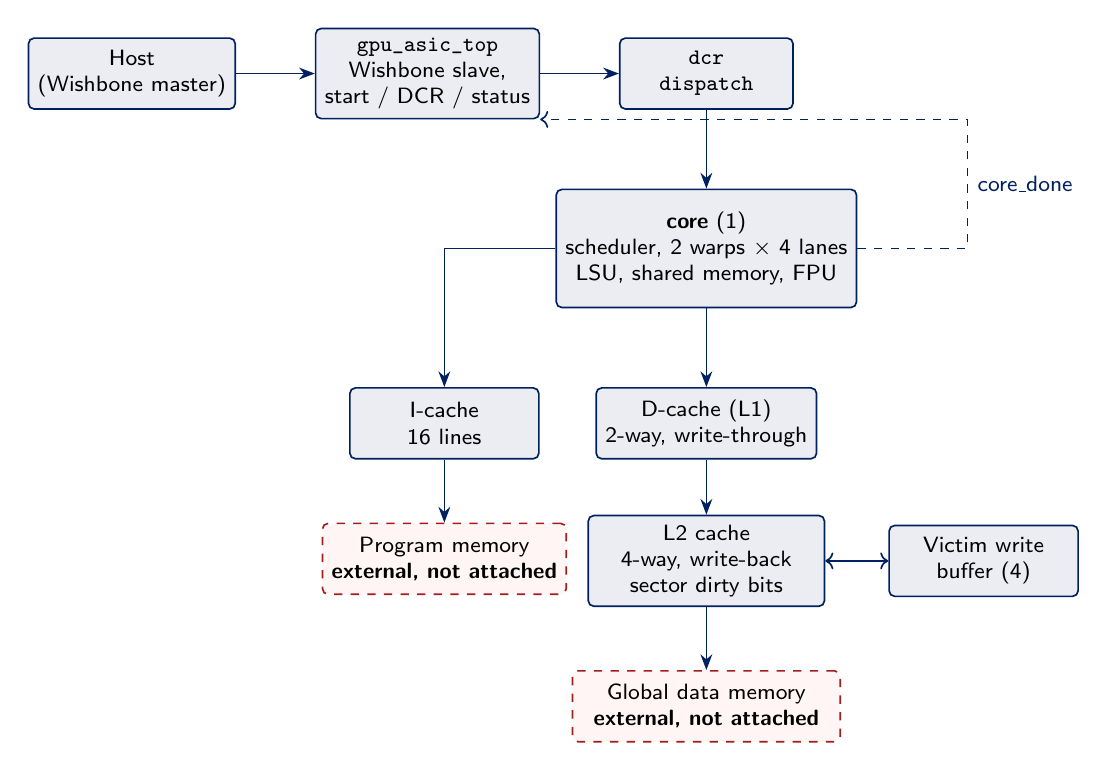
\begin{tikzpicture}[font=\sffamily\footnotesize,
  blk/.style={draw=navy,fill=navy!8,rounded corners=2pt,minimum height=0.9cm,align=center,line width=0.6pt},
  ext/.style={draw=warnred,dashed,fill=red!4,rounded corners=2pt,minimum height=0.9cm,align=center,line width=0.6pt},
  arr/.style={-{Stealth[length=2mm]},line width=0.6pt,color=navy}]
 \node[blk,minimum width=2.4cm] (host) {Host\\(Wishbone master)};
 \node[blk,right=1.0cm of host,minimum width=2.6cm] (top) {\sig{gpu_asic_top}\\Wishbone slave,\\start / DCR / status};
 \node[blk,right=1.0cm of top,minimum width=2.2cm] (disp) {\sig{dcr}\\\sig{dispatch}};
 \node[blk,below=1.0cm of disp,minimum width=3.6cm,minimum height=1.5cm] (core) {\textbf{core} (1)\\scheduler, 2 warps $\times$ 4 lanes\\LSU, shared memory, FPU};
 \node[blk,below left=1.0cm and 0.2cm of core,minimum width=2.4cm] (ic) {I-cache\\16 lines};
 \node[blk,below=1.0cm of core,minimum width=2.4cm] (dc) {D-cache (L1)\\2-way, write-through};
 \node[blk,below=0.7cm of dc,minimum width=3.0cm] (l2) {L2 cache\\4-way, write-back\\sector dirty bits};
 \node[blk,right=0.8cm of l2,minimum width=2.4cm] (vwb) {Victim write\\buffer (4)};
 \node[ext,below=0.8cm of ic,minimum width=3.0cm] (pm) {Program memory\\\textbf{external, not attached}};
 \node[ext,below=0.8cm of l2,minimum width=3.4cm] (dm) {Global data memory\\\textbf{external, not attached}};
 \draw[arr] (host) -- (top); \draw[arr] (top) -- (disp); \draw[arr] (disp) -- (core);
 \draw[arr] (core) -| (ic); \draw[arr] (core) -- (dc); \draw[arr] (dc) -- (l2);
 \draw[arr,<->] (l2) -- (vwb); \draw[arr] (ic) -- (pm); \draw[arr] (l2) -- (dm);
 \draw[arr,->,dashed] (core.east) -- ++(1.4,0) |- (top.south east) node[pos=0.25,right]{core\_done};
\end{tikzpicture}
\caption{System block diagram of the ASIC profile. Dashed red boxes mark interfaces that exist in the RTL but are tied off in \sig{gpu_asic_top} (erratum L3).}
\end{figure}
The I-cache has its own path to the program-memory controller and does \emph{not} pass through the L2.
Both memory interfaces use a native 128-bit block protocol (valid/ready/address/data/strobe) through
\sig{controller.sv}. An AXI4 adaptor exists in the repository but is \textbf{not} instantiated in the ASIC top level.

\section{Host interface: Wishbone slave}
\sig{gpu_asic_top} is a 32-bit Wishbone classic slave with a registered, single-cycle acknowledge
(\sig{wb_ack_o} rises one clock after a request with both \sig{wb_cyc_i} and \sig{wb_stb_i} set).

\begin{table}[ht]\centering\rowcol
\begin{tabular}{@{}llll@{}}
\tblhead{Signal} & \tblhead{Dir} & \tblhead{Width} & \tblhead{Function}\\
\sig{clk}, \sig{reset} & in & 1, 1 & clock, synchronous reset\\
\sig{wb_cyc_i}, \sig{wb_stb_i}, \sig{wb_we_i} & in & 1 each & cycle, strobe, write enable\\
\sig{wb_sel_i} & in & 4 & byte select (\emph{ignored} by the RTL)\\
\sig{wb_adr_i} & in & 32 & address (only bits [15:12] and [7:0] decoded)\\
\sig{wb_dat_i} & in & 32 & write data\\
\sig{wb_dat_o} & out & 32 & read data (registered)\\
\sig{wb_ack_o} & out & 1 & acknowledge\\
\sig{gpu_done_pin} & out & 1 & mirrors the \sig{done} status bit\\
\bottomrule
\end{tabular}
\caption{Pins of \sig{gpu_asic_top}: 107 signal pins in total (73 inputs, 34 outputs), excluding power.}
\end{table}

\subsection{Register map}
The intended base address is \texttt{0x3000\_0000}. The decoder uses only \sig{wb_adr_i[15:12]==0} and \sig{wb_adr_i[7:0]};
the upper address bits are not compared, so the registers alias throughout the 4\,GiB space unless the surrounding
interconnect decodes the base. Accesses to undecoded offsets are acknowledged and read as the previous \sig{wb_dat_o}.

\begin{table}[ht]\centering\rowcol
\begin{tabular}{@{}lllp{8.4cm}@{}}
\tblhead{Address} & \tblhead{Access} & \tblhead{Name} & \tblhead{Description}\\
\texttt{0x3000\_0000} & W & CTRL & \texttt{[0]} START (level; stays set until written 0); \texttt{[15:8]} THREAD\_COUNT (total threads to launch, written to internal DCR 0x00); other bits ignored\\
\texttt{0x3000\_0000} & R & CTRL & \texttt{\{16'b0, THREAD\_COUNT[7:0], 7'b0, START\}}\\
\texttt{0x3000\_0004} & R & STATUS & \texttt{[0]} DONE; \texttt{[31:1]} 0\\
\texttt{0x3000\_1000}--\texttt{1FFF} & --- & \emph{unified memory window} & \textbf{Not implemented} (described in a source comment only; erratum L3)\\
\bottomrule
\end{tabular}
\caption{Wishbone register map as implemented (\sig{gpu_asic_top.sv:55-70}).}
\end{table}

\subsection{Internal Device Control Register (DCR) block}
The DCR (\sig{dcr.sv}) has an 8-bit address / 8-bit data write port. \textbf{Only address \texttt{0x00} is reachable from the
chip pins}: the Wishbone wrapper always drives address \texttt{0x00} (erratum L13). The remaining registers exist for
integration and simulation.

\begin{table}[ht]\centering\rowcol
\begin{tabular}{@{}llp{9.6cm}@{}}
\tblhead{DCR addr} & \tblhead{Name} & \tblhead{Function}\\
\texttt{0x00} & THREAD\_COUNT & total threads in the launch (8-bit, reset 0)\\
\texttt{0x01} & PMU\_RESET & one-cycle pulse: clear all PMU counters\\
\texttt{0x02} & PMU\_SNAPSHOT & one-cycle pulse: latch counters into snapshot registers\\
\texttt{0x10}--\texttt{0x13} & PMU\_CFG0--3 & 5-bit event selector for counter 0--3 (see Appendix~\ref{app:pmu})\\
\bottomrule
\end{tabular}
\end{table}

\section{Address spaces}
\begin{table}[ht]\centering\rowcol
\begin{tabular}{@{}p{2.8cm}p{3.1cm}p{2.2cm}p{7.6cm}@{}}
\tblhead{Space} & \tblhead{Size / width} & \tblhead{Access} & \tblhead{Notes}\\
Program memory & 4\,K words, 12-bit PC & fetch only & word-addressed; I-cache fetches 4-word blocks; external memory required\\
Global data & 16\,K words, 14-bit address & \ins{LDR STR ATOM_*} & word-addressed; the core faults accesses above \texttt{0xFFFF}, but the bus carries only 14 bits, so \texttt{0x4000}--\texttt{0xFFFF} \textbf{silently alias} (L14)\\
Shared memory & 64 words & \ins{LDSH STSH} & per-core, shared by all 8 threads; bank = \texttt{addr[1:0]}; fault if address $\ge$ 64\\
Host MMIO & 2 registers & Wishbone & \S2.2\\
\bottomrule
\end{tabular}
\caption{Address spaces of the ASIC profile.}
\end{table}

\section{Reset and launch sequence}
\begin{enumerate}[leftmargin=1.4em,itemsep=1pt]
\item Assert \sig{reset}, then release.
\item Host writes CTRL with START=1 and THREAD\_COUNT in bits [15:8]. START and the DCR write occur in the same bus cycle.
\item The dispatcher computes $\lceil \text{THREAD\_COUNT}/8\rceil$ blocks. With one core, \textbf{blocks run sequentially}:
 each block resets the core and launches 8 threads (the last block may be partial); \reg{29} holds the block id.
\item When all blocks have finished, the dispatcher raises \sig{flush_caches}; the D-cache invalidates and the L2 writes all dirty sectors back
 through the victim buffer. DONE is set only after every flush completes, so external memory is coherent when DONE reads 1.
\item DONE clears when the host writes START=0 and the dispatcher is idle. By code inspection (not simulated), holding START=1 after DONE re-triggers the flush loop, so software should drop START after observing DONE.
\end{enumerate}

% =============================================================================
\chapter{Core microarchitecture}\label{ch:core}
% =============================================================================
\section{Pipeline}
\begin{table}[ht]\centering\rowcol
\begin{tabular}{@{}lp{3.3cm}p{10.4cm}@{}}
\tblhead{Stage} & \tblhead{Module(s)} & \tblhead{Function}\\
IF & \sig{fetcher}, \sig{icache} & 3-state FSM (IDLE, FETCHING, DONE) fetching one instruction at a time for the warp chosen by the scheduler. The held instruction is tagged with the PC it was fetched for (\sig{fetched_pc}); it is accepted only if that PC equals the PC of the warp being issued, otherwise the fetcher drops it and refetches.\\
ID & \sig{decoder}, ID latch & Combinational decode; the \sig{id_*} latch registers instruction, PC, warp id and active mask. Register-file read with write-through bypass. A flush of the previous occupant's warp squashes the latch only if no fresh instruction is loading in the same cycle.\\
EX & \sig{alu}, \sig{fp32_fma}, \sig{pc} (per lane) & Per-lane integer ALU and FMA, forwarding network (MEM, WB and LSU-return sources), NZP update, next-PC computation, branch/divergence/exception detection.\\
MEM & \sig{lsu}, \sig{shared_mem} & Memory instructions engage the LSU; the issuing warp parks in \texttt{WAITING\_MEM} until its lanes complete. Other instructions pass through.\\
WB & \sig{registers} & Three writers with fixed priority: FP writeback $>$ LSU return $>$ integer ALU.\\
\bottomrule
\end{tabular}
\caption{Pipeline stages.}
\end{table}

\section{Datapath}
\begin{figure}[ht]\centering
\resizebox{\linewidth}{!}{%
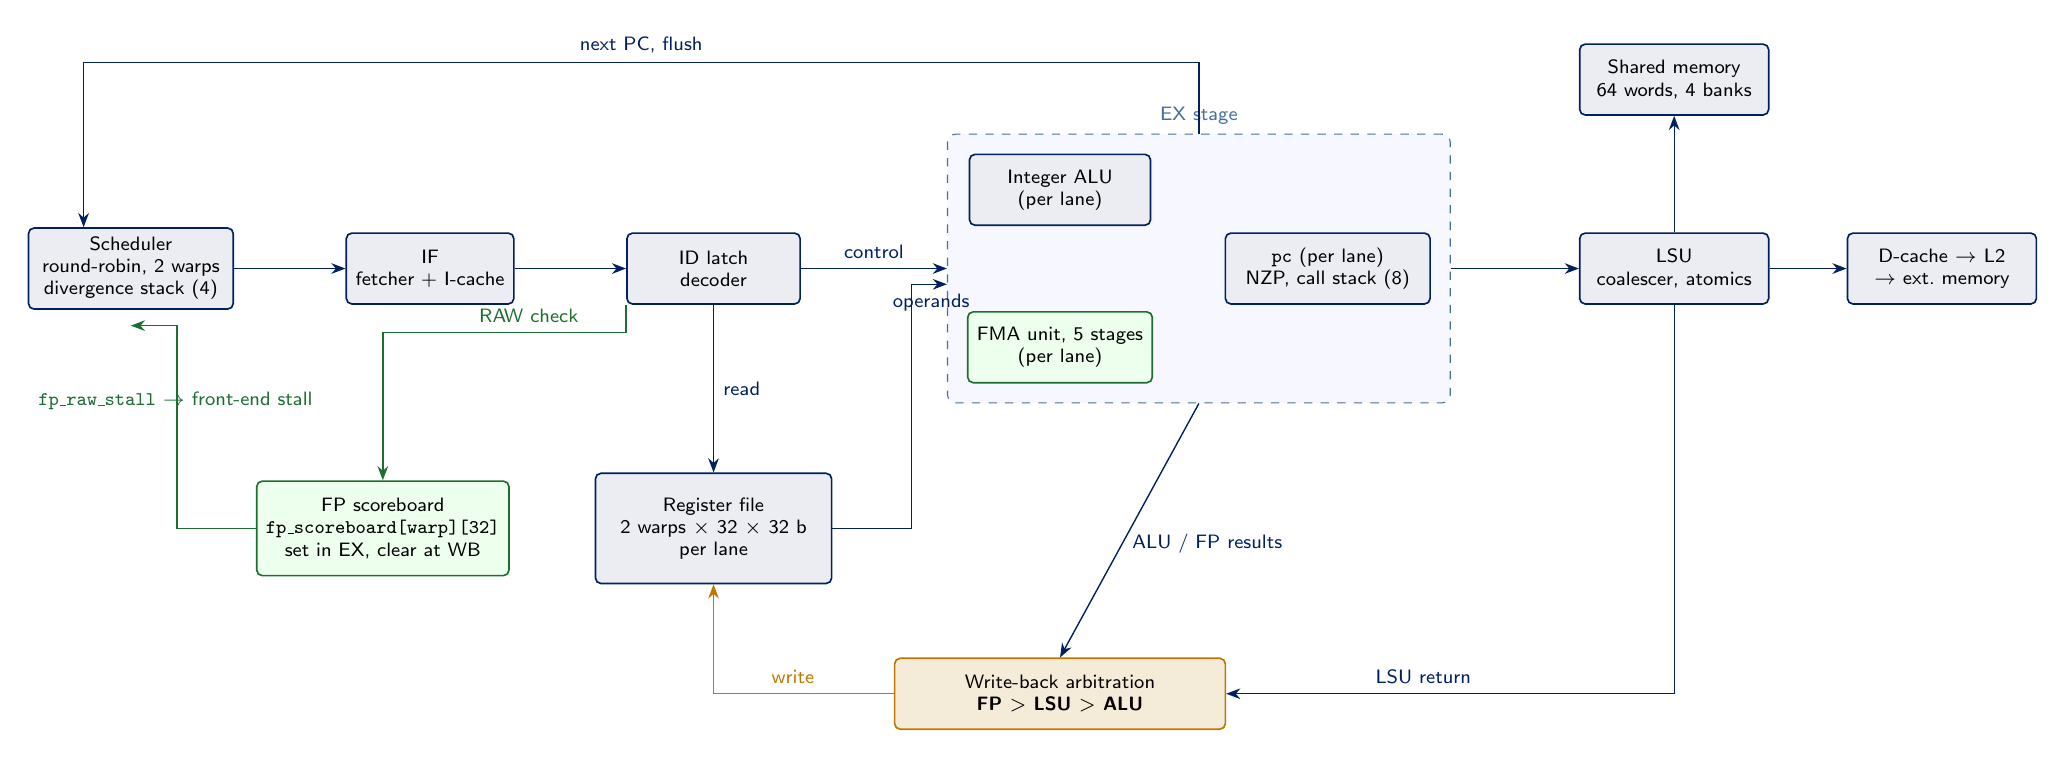
\begin{tikzpicture}[font=\sffamily\scriptsize,
  blk/.style={draw=navy,fill=navy!8,rounded corners=2pt,minimum height=0.9cm,align=center,line width=0.6pt},
  fp/.style={draw=okgreen,fill=green!7,rounded corners=2pt,minimum height=0.9cm,align=center,line width=0.6pt},
  arr/.style={-{Stealth[length=1.8mm]},line width=0.5pt,color=navy},
  garr/.style={-{Stealth[length=1.8mm]},line width=0.5pt,color=okgreen}]
 \node[blk,minimum width=2.6cm] (sch) at (0,3) {Scheduler\\round-robin, 2 warps\\divergence stack (4)};
 \node[blk,minimum width=2.0cm] (if) at (3.8,3) {IF\\fetcher + I-cache};
 \node[blk,minimum width=2.2cm] (id) at (7.4,3) {ID latch\\decoder};
 \node[blk,minimum width=3.0cm,minimum height=1.4cm] (rf) at (7.4,-0.3) {Register file\\2 warps $\times$ 32 $\times$ 32 b\\per lane};
 \node[fp,minimum width=2.8cm,minimum height=1.2cm] (sb) at (3.2,-0.3) {FP scoreboard\\\texttt{fp\_scoreboard[warp][32]}\\set in EX, clear at WB};
 \node[blk,minimum width=2.3cm] (alu) at (11.8,4.0) {Integer ALU\\(per lane)};
 \node[fp,minimum width=2.3cm] (fma) at (11.8,2.0) {FMA unit, 5 stages\\(per lane)};
 \node[blk,minimum width=2.6cm] (pcb) at (15.2,3.0) {\texttt{pc} (per lane)\\NZP, call stack (8)};
 \begin{scope}[on background layer]
  \node[draw=steel,dashed,fill=blue!3,rounded corners=3pt,fit=(alu)(fma)(pcb),inner sep=7pt,label={[font=\sffamily\scriptsize,text=steel]above:EX stage}] (ex) {};
 \end{scope}
 \node[blk,minimum width=2.4cm] (lsu) at (19.6,3.0) {LSU\\coalescer, atomics};
 \node[blk,minimum width=2.4cm] (shm) at (19.6,5.4) {Shared memory\\64 words, 4 banks};
 \node[blk,minimum width=2.4cm] (l1) at (23.0,3.0) {D-cache $\rightarrow$ L2\\$\rightarrow$ ext.\ memory};
 \node[blk,minimum width=4.2cm,fill=amber!15,draw=amber] (wb) at (11.8,-2.4) {Write-back arbitration\\\textbf{FP $>$ LSU $>$ ALU}};
 \draw[arr] (sch) -- (if); \draw[arr] (if) -- (id);
 \draw[arr] (id.east) -- (ex.west |- id.east) node[pos=0.5,above]{control};
 \draw[arr] (id.south) -- (rf.north) node[pos=0.5,right]{read};
 \draw[arr] (rf.east) -- ++(1.0,0) |- ([yshift=-2mm]ex.west) node[pos=0.78,below]{operands};
 \draw[garr] (id.south west) -- ++(0,-0.35) -| (sb.north) node[pos=0.2,above]{RAW check};
 \draw[garr] (sb.west) -- ++(-1.0,0) |- ([yshift=-0.2cm]sch.south) ;
 \draw[arr] (ex.east) -- (lsu.west |- ex.east);
 \draw[arr] (lsu.north) -- (shm.south); \draw[arr] (lsu.east) -- (l1.west);
 \draw[arr] (ex.north) -- ++(0,0.9) -| ([xshift=-0.6cm]sch.north) node[pos=0.25,above]{next PC, flush};
 \draw[arr] (ex.south) -- (wb.north) node[pos=0.55,right]{ALU / FP results};
 \draw[arr] (lsu.south) |- (wb.east) node[pos=0.78,above]{LSU return};
 \draw[arr,color=amber] (wb.west) -| (rf.south) node[pos=0.28,above]{write};
 \node[font=\sffamily\scriptsize,text=okgreen,anchor=north west] at (-1.3,1.55) {\texttt{fp\_raw\_stall} $\rightarrow$ front-end stall};
\end{tikzpicture}}
\caption{Core datapath. Blue: instruction/operand flow; green: FP hazard control; amber: write-back arbitration into the register file.}
\end{figure}

\section{Warp scheduler}
The scheduler (\sig{scheduler.sv}) selects, every cycle and combinationally, the next \texttt{READY} warp with a non-empty
active mask, round-robin from \sig{rr_ptr}, excluding warps that are being flushed in the same cycle.
Warp states: \texttt{IDLE, READY, WAITING\_MEM, WAITING\_BARRIER, WAITING\_FP, DONE\_STATE, FAULTED}.
Branch, call, divergence and exception outcomes are resolved in EX and redirect the front end through a one-cycle
per-warp pulse \sig{flush_warp_mask}; the squashed instructions are those between fetch and EX for that warp.

\subsection{Divergence handling (SIMT stack)}
Each warp has a 4-entry stack of \texttt{(PC, active\_mask)} (\sig{scheduler.sv:57-65}). In EX, the next PC of every active
lane is computed. If all lanes agree, the warp continues. If they disagree, the lanes are split into two groups: group~A
(the group containing the lowest active lane) continues, and group~B's \texttt{(target, mask)} is pushed.
\begin{itemize}[leftmargin=1.4em,itemsep=1pt]
\item \textbf{Reconvergence} happens when a non-divergent branch of the running group targets \emph{exactly} the PC on top of the stack:
 the entry is popped and the masks are merged.
\item At \texttt{EXIT}, a non-empty stack is popped and the saved group resumes at its saved PC.
\item There is \textbf{no} reconvergence at a join point or post-dominator. In practice lane groups run the remainder of the program serially
 until \texttt{EXIT}. Results are correct; barriers are not (\S\ref{sec:restrictions}, erratum L1).
\end{itemize}
Maximum nesting is lane-count minus one (3 for four lanes), which fits the 4-entry stack. A profile with more than five lanes could overflow it (L7).

\subsection{Call/return stack}
Return addresses are held by each lane's \sig{pc} instance: 8 entries per warp with a 3-bit pointer
(\sig{pc.sv:29-33}). \ins{CALL} pushes \texttt{PC+1} and jumps to the absolute target; \ins{RET_FN} pops. There is
\textbf{no overflow or underflow detection}: the ninth nested call wraps the pointer and overwrites the oldest return
address (erratum L6, demonstrated by \texttt{make limits}).

\section{Floating-point unit}
Each lane has a private \sig{fp32_fma} with a fixed \textbf{5-cycle} latency from the EX stage to the register write.
\begin{table}[ht]\centering\rowcol
\begin{tabular}{@{}lll@{}}
\tblhead{Instruction} & \tblhead{Internal operation $(a\cdot b)+c$} & \tblhead{Result}\\
\ins{FMA}  & $a\cdot b + c$ with $a{=}\texttt{rs},\ b{=}\texttt{rt},\ c{=}\texttt{rd}$ & $\texttt{rs}\times\texttt{rt}+\texttt{rd}$\\
\ins{FADD} & $a\cdot 1.0 + b$ & $\texttt{rs}+\texttt{rt}$\\
\ins{FMUL} & $a\cdot b + 0$ & $\texttt{rs}\times\texttt{rt}$\\
\ins{FSUB} & $a\cdot 1.0 + (-b)$ & $\texttt{rs}-\texttt{rt}$\\
\bottomrule
\end{tabular}
\end{table}
Pipeline stages: (1) mantissa multiply and exponent add, (2a) alignment, (2b) add/subtract with sign selection,
(3) normalisation (leading-one detect), (4) pack. Numerics (this is \emph{not} full IEEE-754; erratum L8):
\begin{itemize}[leftmargin=1.4em,itemsep=1pt]
\item results are \textbf{truncated} (no rounding); denormal inputs read as zero and results below the normal range flush to $\pm0$;
\item exponent 255 is treated as an ordinary exponent (no NaN/Inf propagation); overflow produces an infinity \emph{encoding};
\item the product exponent is computed even when an operand is zero, so $0\times 2^{127}+c$ drops low mantissa bits of $c$;
\item exact cancellation yields a zero carrying the sign of the product term ($a\cdot b$).
\end{itemize}

\subsection{Scoreboard and hazards}
\sig{fp_scoreboard[warp][reg]} is a 32-bit-per-warp vector. An FP instruction sets its destination bit when it fires in EX; the bit
clears when the result reaches write-back (fifth cycle). The ID stage compares the instruction's \texttt{rs}, \texttt{rt} and
(when read) \texttt{rd} with the scoreboard; a hit raises \sig{fp_raw_stall}, which stalls the front end and squashes the EX
latch for that cycle. In addition, when an FP instruction reaches EX the \emph{warp} is parked in \texttt{WAITING\_FP} and its
younger instructions are flushed (\sig{scheduler.sv:193-197}); it resumes when its FP result is written back. Other warps keep issuing.

\subsection{Register-file write arbitration}
Priority 1 FP write-back, priority 2 LSU return, priority 3 integer ALU (\sig{registers.sv}); lower priorities are suppressed when the
same warp \emph{and} register collide. Writes to \reg{29}--\reg{31} are ignored by all writers.
\begin{notebox}{Why the ALU-versus-FP collision guard cannot be exercised}
Removing the ALU-side FP-collision guard in a mutation experiment was \emph{not} detected by 100 random programs. The design reason is
that an FP operation parks its own warp in \texttt{WAITING\_FP} and flushes its younger instructions, while older instructions have left the
pipeline before the five-cycle FP result returns, so an ALU write to the same warp/register cannot coincide with the FP write-back.
This is a design argument supported by the 0/100 mutation survival; it has \textbf{not} been formally proven.
\end{notebox}

\section{Memory subsystem}
\subsection{Load/store unit and coalescing}
The LSU (\sig{lsu.sv}) accepts one memory instruction per warp and works through the active lanes with a state machine
(\texttt{IDLE, COALESCE\_READ, WAIT\_READ, COALESCE\_WRITE, WAIT\_WRITE, WAIT\_SHARED, ATOMIC\_*}).
\begin{itemize}[leftmargin=1.4em,itemsep=1pt]
\item \textbf{Reads:} the lowest pending lane selects a 128-bit block; every pending lane whose word lies in that block is served by the same
 transaction. Lanes in other blocks need further transactions.
\item \textbf{Writes:} all pending lanes that map to the selected block are packed into one 128-bit beat with a 4-bit word strobe,
 so contiguous lane addresses produce a single block write.
\item \textbf{Atomics} (\ins{ATOM_ADD}, \ins{ATOM_CAS}) are serialised lane by lane: read the block, apply the operation, write back one word,
 return the old value in \texttt{rd}.
\item The effective address is \texttt{rs + sign\_extend(imm16)} for \ins{LDR}/\ins{STR}; atomics and shared-memory accesses use \texttt{rs} alone.
\end{itemize}

\subsection{Banked shared memory}
64 words in 4 banks of 16 words: \texttt{bank = addr[1:0]}, \texttt{offset = addr[5:2]}. Every lane has its own request port.
Per cycle, lanes are processed in index order and a lane is deferred (not dropped) if
\begin{itemize}[leftmargin=1.4em,itemsep=1pt]
\item \emph{write bank conflict}: a lower lane writes the same bank in the same cycle;
\item \emph{read bank conflict}: a lower lane reads the same bank at a \emph{different} address;
\item \emph{read-after-write}: a lower lane writes the address being read.
\end{itemize}
Lanes reading the \emph{same} address as a lower lane are served by \textbf{multicast broadcast} (they copy the data fetched for that lower lane).
Shared memory resets to zero. The memory is shared by all warps of the core; ordering between warps requires \ins{SYNC}.

\subsection{Caches and victim write buffer}
\begin{table}[ht]\centering\rowcol
\begin{tabular}{@{}p{2.6cm}p{5.0cm}p{8.1cm}@{}}
\tblhead{Level} & \tblhead{Organisation} & \tblhead{Policy}\\
I-cache & 16 lines, direct-mapped, 4-word lines & read-only; miss fetches the block from the program controller\\
D-cache (L1) & 16 lines = 8 sets $\times$ 2 ways, LRU bit & \textbf{write-through}; write hit merges into the line, write miss does not allocate; read miss allocates\\
L2 & 64 lines = 16 sets $\times$ 4 ways, 3-bit PLRU, 4 sectors of 32 bit per line with per-sector dirty bits & \textbf{write-back, write-allocate}; evicting a dirty line pushes it into the victim write buffer\\
Victim write buffer & 4 entries (128-bit data + 4 dirty bits) & merges pushes to the same address (dirty-sector merge); drains when half full, on a flush, or after an idle timeout (31 cycles); an L2 miss that hits the buffer is served from it and the entry is popped (probe-hit bypass)\\
\bottomrule
\end{tabular}
\caption{Cache hierarchy (ASIC profile).}
\end{table}
The L2 must not push to a full buffer: a push is attempted only when the buffer reports space \emph{and} no push is already in flight
(this handshake was a bug, B4, Chapter~\ref{ch:verif}); the buffer additionally asserts an error if a push ever arrives while full.
At the end of a launch the D-cache is invalidated and the L2 flushed, after which external memory holds all results.

\section{Exceptions}
Division by zero and out-of-range addresses (global $>$\texttt{0xFFFF}, shared $\ge$64) mark the offending warp \texttt{FAULTED} and flush it.
A faulted warp counts as finished for DONE. The core latches \sig{exception_raised/warp/pc/cause}, but \textbf{these signals are not
connected above the core}, so a fault is invisible to the host (erratum L12).

\section{Performance monitoring unit}
Four 32-bit counters, each selecting one of 32 event lines (Appendix~\ref{app:pmu}) through DCR 0x10--0x13, with reset and snapshot pulses.
L2 hit/miss events read zero (L4), and the PMU registers are not reachable from the Wishbone interface (L13).

% =============================================================================
\chapter{Instruction set architecture}\label{ch:isa}
% =============================================================================
\section{Instruction formats}
All instructions are 32 bits. The opcode occupies bits [31:26].
\subsection*{R-type (register--register)}
\bitfield{6/31/26/opcode/steel, 5/25/21/rd/navy, 5/20/16/rs/navy, 5/15/11/rt/navy, 11/10/0/unused (0)/gray}
\subsection*{I-type (immediate, memory)}
\bitfield{6/31/26/opcode/steel, 5/25/21/rd/navy, 5/20/16/rs/navy, 16/15/0/imm16 (sign-extended)/orange}
\subsection*{Branch type (\ins{BRnzp}, \ins{CALL})}
\bitfield{6/31/26/opcode (1)/steel, 3/25/23/nzp/purple, 7/22/16/unused/gray, 16/15/0/absolute target PC/orange}
\ins{CALL} uses opcode 13 with bits [25:16] unused. \ins{RET_FN}, \ins{EXIT}, \ins{SYNC} and \ins{NOP} carry only the opcode.
\subsection*{Load-upper-immediate (\ins{LUI})}
\bitfield{6/31/26/opcode (29)/steel, 5/25/21/rd/navy, 20/20/1/imm20/orange, 1/0/0/--/gray}
\texttt{rd = imm20 << 12}.

\begin{notebox}{Operand-slot conventions}
For \ins{STR} and \ins{STSH} the register holding the \emph{value to store} is encoded in the \texttt{rd} field and the address register in \texttt{rs}
(the decoder re-routes the \texttt{rd} slot into the second source). For \ins{MAC}, \ins{FMA} and \ins{ATOM_CAS}, \texttt{rd} is also an input.
\ins{BRnzp} encodes the condition in \texttt{[25:23]} as \texttt{N=bit\,25, Z=bit\,24, P=bit\,23}.
\end{notebox}

\section{Register file conventions}
\begin{table}[ht]\centering\rowcol
\begin{tabular}{@{}lllp{8.3cm}@{}}
\tblhead{Register} & \tblhead{Name} & \tblhead{Access} & \tblhead{Value / convention}\\
\reg{0}--\reg{28} & general purpose & R/W & reset to 0; no ABI is imposed by the hardware\\
\reg{29} & \texttt{blockIdx} & R, writes ignored & block id assigned by the dispatcher (8 bits, zero-extended)\\
\reg{30} & \texttt{blockDim} & R, writes ignored & \texttt{THREADS\_PER\_BLOCK $\times$ NUM\_WARPS} = \textbf{8} (threads per block)\\
\reg{31} & \texttt{threadIdx} & R, writes ignored & \texttt{warp\_id $\times$ 4 + lane} (0--7)\\
\bottomrule
\end{tabular}
\caption{Per-thread register file. Global thread id: \texttt{MUL R0,R29,R30 ; ADD R0,R0,R31}.}
\end{table}
Each lane holds 2 warps $\times$ 32 = 64 registers. The register file is written by up to three sources per cycle (Chapter~\ref{ch:core}); a write-through bypass forwards a value to a same-cycle read of the same warp.

\section{Instruction reference}
\textit{Notation:} \texttt{rd, rs, rt} are registers, \texttt{imm} a 16-bit signed immediate, \texttt{T} an absolute program address.
Integer values are 32-bit two's complement unless stated.

\subsection{Integer arithmetic and logic}
\rowcol
\begin{longtable}{@{}lrp{3.3cm}p{9.0cm}@{}}
\tblhead{Mnemonic} & \tblhead{Op} & \tblhead{Operands} & \tblhead{Behaviour}\\\endhead
\ins{ADD}  & 3  & rd, rs, rt & $rd = rs + rt$ (wraps)\\
\ins{SUB}  & 4  & rd, rs, rt & $rd = rs - rt$ (wraps)\\
\ins{MUL}  & 5  & rd, rs, rt & low 32 bits of the signed product\\
\ins{DIV}  & 6  & rd, rs, rt & unsigned quotient; \texttt{rt=0} faults. \textbf{Returns 0 unless built with \texttt{USE\_COMB\_DIV}} (L2)\\
\ins{MOD}  & 22 & rd, rs, rt & unsigned remainder; same caveats as \ins{DIV}\\
\ins{AND}  & 17 & rd, rs, rt & bitwise AND\\
\ins{OR}   & 18 & rd, rs, rt & bitwise OR\\
\ins{XOR}  & 19 & rd, rs, rt & bitwise XOR\\
\ins{SHL}  & 20 & rd, rs, rt & logical left shift by \texttt{rt}; counts $\ge32$ give 0\\
\ins{SHR}  & 21 & rd, rs, rt & logical right shift; counts $\ge32$ give 0\\
\ins{MIN}  & 23 & rd, rs, rt & signed minimum\\
\ins{MAX}  & 24 & rd, rs, rt & signed maximum\\
\ins{ABS}  & 25 & rd, rs & signed absolute value ($\texttt{0x80000000}\mapsto\texttt{0x80000000}$)\\
\ins{NEG}  & 26 & rd, rs & two's-complement negate\\
\ins{MAC}  & 27 & rd, rs, rt & $rd = rd + rs\cdot rt$ (signed, low 32 bits); reads \texttt{rd}\\
\ins{POPCNT} & 30 & rd, rs & number of set bits\\
\ins{CLZ}  & 31 & rd, rs & leading zeros ($\mathrm{CLZ}(0)=32$)\\
\ins{BREV} & 32 & rd, rs & bit reversal\\
\ins{CONST} & 9 & rd, imm & $rd = \mathrm{sext}(imm16)$\\
\ins{LUI}  & 29 & rd, imm20 & $rd = imm20 \ll 12$\\
\bottomrule
\end{longtable}
The ALU also computes carry, overflow, zero, negative and saturation flags, but \textbf{no instruction reads them}.

\subsection{Floating point (single precision)}
\rowcol
\begin{longtable}{@{}lrp{3.3cm}p{9.0cm}@{}}
\tblhead{Mnemonic} & \tblhead{Op} & \tblhead{Operands} & \tblhead{Behaviour}\\\endhead
\ins{FADD} & 33 & rd, rs, rt & $rd = rs + rt$\\
\ins{FSUB} & 34 & rd, rs, rt & $rd = rs - rt$\\
\ins{FMUL} & 35 & rd, rs, rt & $rd = rs \times rt$\\
\ins{FMA}  & 36 & rd, rs, rt & $rd = rs\times rt + rd$ (reads \texttt{rd}); single rounding point: truncation\\
\bottomrule
\end{longtable}

\subsection{Compare, branch and call}
\rowcol
\begin{longtable}{@{}lrp{3.3cm}p{9.0cm}@{}}
\tblhead{Mnemonic} & \tblhead{Op} & \tblhead{Operands} & \tblhead{Behaviour}\\\endhead
\ins{CMP}    & 2  & rs, rt & sets this lane's NZP flags: \texttt{N = rs<rt, Z = rs==rt, P = rs>rt} using an \textbf{unsigned} comparison (L5). Writes no register\\
\ins{BRnzp}  & 1  & nzp, T & taken iff $(\mathrm{NZP}\ \&\ \mathrm{nzp})\neq0$. NZP is 0 after reset, so a branch before any \ins{CMP} falls through even with \texttt{nzp=111}\\
\ins{CALL}   & 13 & T & push \texttt{PC+1} on the lane's return stack, jump to \texttt{T}\\
\ins{RET_FN} & 14 & --- & pop the return stack and jump (undefined if empty)\\
\ins{EXIT}   & 15 & --- & terminate the lane; if the warp's divergence stack is non-empty the next group resumes\\
\ins{NOP}    & 0  & --- & no operation\\
\bottomrule
\end{longtable}

\subsection{Memory, shared memory and atomics}
\rowcol
\begin{longtable}{@{}lrp{3.3cm}p{9.0cm}@{}}
\tblhead{Mnemonic} & \tblhead{Op} & \tblhead{Operands} & \tblhead{Behaviour}\\\endhead
\ins{LDR}  & 7  & rd, [rs+imm] & load word from global memory; fault if address $>$\texttt{0xFFFF}; addresses $\ge$\texttt{0x4000} alias (L14)\\
\ins{STR}  & 8  & rv, [rs+imm] & store \texttt{rv} (encoded in the rd slot) to global memory\\
\ins{LDSH} & 11 & rd, [rs] & load from shared memory (no offset); fault if address $\ge64$\\
\ins{STSH} & 12 & rv, [rs] & store \texttt{rv} (rd slot) to shared memory\\
\ins{ATOM_ADD} & 16 & rd, rs, rt & $\texttt{old}=\texttt{mem}[rs];\ \texttt{mem}[rs]=\texttt{old}+rt;\ rd=\texttt{old}$; lanes serialised\\
\ins{ATOM_CAS} & 28 & rd, rs, rt & $\texttt{old}=\texttt{mem}[rs]$; if $\texttt{old}=rd$ then $\texttt{mem}[rs]=rt$; $rd=\texttt{old}$ (\texttt{rd} is both compare input and result)\\
\bottomrule
\end{longtable}

\subsection{Synchronisation}
\rowcol
\begin{longtable}{@{}lrp{3.3cm}p{9.0cm}@{}}
\tblhead{Mnemonic} & \tblhead{Op} & \tblhead{Operands} & \tblhead{Behaviour}\\\endhead
\ins{SYNC} & 10 & --- & block barrier (\texttt{\_\_syncthreads()}): the warp waits until every non-finished warp of the core has executed \ins{SYNC}. \textbf{Requires warp-uniform control flow} (\S\ref{sec:restrictions})\\
\bottomrule
\end{longtable}
Opcodes 37--63 are reserved and decode as inert instructions.

\section{Programming example}
The following program is the instruction sequence of a branch/call test; the encodings were generated by the project's assembler functions
(\sig{scripts/isa.py}) and executed on the RTL.
\begin{lstlisting}[style=asm]
 0:  24200007  CONST R1, 7
 1:  145f0800  MUL   R2, R31, R1      ; R2 = threadIdx * 7
 2:  08020800  CMP   R2, R1           ; N/Z/P = R2 <,==,> R1 (unsigned)
 3:  04800005  BRp   5                ; skip the call when R2 > R1
 4:  34000007  CALL  7
 5:  205f012c  STR   R2, [R31+300]    ; mem[300+tid] = R2
 6:  3c000000  EXIT
 7:  0c420800  ADD   R2, R2, R1       ; callee
 8:  38000000  RET_FN
\end{lstlisting}

\section{Architectural restrictions and hazards}\label{sec:restrictions}
\begin{warnbox}{R1 --- \ins{SYNC} requires warp-uniform control flow}
The barrier is tracked at \textbf{warp} granularity: when a lane group executes \ins{SYNC}, the warp enters \texttt{WAITING\_BARRIER} and is counted once
(\sig{barrier_count >= num_active_warps_comb}, \sig{scheduler.sv:272}). Because divergent lane groups are serialised until \ins{EXIT} (no join-point reconvergence),
a \ins{SYNC} that follows divergent code is executed once \emph{per group}, and the first group to arrive releases the barrier while other lanes have not yet
performed their stores. Result: threads can read stale shared memory (observed: 4 of 8 threads in the directed test, and in 18 of 240 early random programs).
\textbf{Rule:} every branch and loop bound that precedes a \ins{SYNC} must be uniform across the warp (derived from constants, \reg{29}, \reg{30}, or the warp id); it may differ \emph{between} warps.
Divergence without barriers is fully supported. A \ins{SYNC} executed after some lanes have already executed \ins{EXIT} is likewise unsupported.
\end{warnbox}
\begin{warnbox}{R2 --- return-stack overflow}
Nesting deeper than 8 \ins{CALL}s wraps the 3-bit stack pointer silently and corrupts the oldest return address; a ninth nested call hangs or mis-returns on the RTL.
\ins{RET_FN} with an empty stack jumps to a stale address. Keep call depth $\le 8$.
\end{warnbox}
\begin{notebox}{Other rules}
\textbf{R3} \ins{CMP} is unsigned. \textbf{R4} A conditional/unconditional \ins{BRnzp} needs a preceding \ins{CMP} (NZP resets to 0); an ``always'' jump is \ins{CMP} of a register with itself followed by \texttt{BR 111}.
\textbf{R5} Do not write \reg{29}--\reg{31}. \textbf{R6} \ins{DIV}/\ins{MOD} need \texttt{USE\_COMB\_DIV} and a non-zero divisor. \textbf{R7} Division by zero and bad addresses kill the warp silently.
\textbf{R8} Results are guaranteed in external memory only after DONE. \textbf{R9} Do not rely on the old value returned by \ins{ATOM_ADD} being a particular order across lanes.
\end{notebox}

% =============================================================================
\chapter{Verification and physical implementation}\label{ch:verif}\label{ch:phys}
% =============================================================================
\section{Verification methodology}
\begin{enumerate}[leftmargin=1.4em,itemsep=1pt]
\item \textbf{Lint:} Verilator \texttt{-Wall} on the sim, ASIC and FPGA profiles; ten baseline warning classes are waived, any new class fails.
\item \textbf{Unit tests} (Verilator, self-checking): ALU (56\,736 vectors, run with and without \texttt{USE\_COMB\_DIV}), decoder (all 64 opcodes), \sig{pc},
 register file, FMA (4\,013 pipelined results against a double-precision reference), D-cache and L2+VWB (random partial-write traffic with random memory latency against a golden memory).
\item \textbf{Directed system tests:} NZP/branch/nested-call test on the ASIC profile; 2-core, 32-thread $5{\times}5$ matrix multiply (CALL/RET, divergence, DIV).
\item \textbf{SVA checkers} bound into the RTL (no source edits): issued PC equals fetched PC, no dropped instruction, return-stack pointer discipline, CMP updates NZP,
 divergence-stack bound, LSU strobe sanity, fetcher overlap, VWB no-push-while-full.
\item \textbf{Golden reference model and constrained-random fuzzing.} A Python interpreter (\sig{Machine} in \sig{isa.py}) executes the same machine words, including a bit-exact port of the FMA datapath.
 The generator (\sig{gen.py}) emits terminating, race-free programs using structured control flow (forward if/else, loops with per-thread or per-warp trip counts, an acyclic call graph),
 integer and FP arithmetic, global and shared memory, \ins{SYNC} barriers and \ins{ATOM_ADD}; each program dumps all registers to memory. The runner (\sig{rand_regress.py}) executes each program on the RTL with randomised memory latency and compares \emph{all} 1024 data words with the model.
 Programs that use barriers are generated in a ``uniform'' mode (restriction R1) with deliberate warp imbalance.
\item \textbf{Limitation characterisation} (\texttt{make limits}) and a \textbf{documentation consistency check} (\texttt{make docs-check}) keep this manual and the repository synchronised.
\end{enumerate}
\texttt{make verify} runs lint, unit, system, a short random run, limitation and documentation checks.

\section{Regression results}
\begin{table}[ht]\centering\rowcol
\begin{tabular}{@{}p{5.9cm}p{4.7cm}p{3.4cm}r@{}}
\tblhead{Campaign (generator content)} & \tblhead{Memory latency (max extra cycles)} & \tblhead{Programs / latency} & \tblhead{Mismatches}\\
Integer, control flow, CALL/RET & 0, 2, 5, 10, 25 & 600 each (3000) & 0\\
+ FP, shared memory, SYNC, atomics & 0, 5, 20 & 1200 each (3600) & 0\\
+ warp-imbalanced barriers (final) & 0, 3, 10, 30 & 800 each (3200) & 0\\
\bottomrule
\end{tabular}
\caption{Constrained-random campaigns on the final RTL (ASIC profile, 8 threads). Each program is 150--300 instructions.}
\end{table}
All 9\,800 runs matched the model bit-for-bit with all SVA checkers enabled. The first campaign pre-dates the FP/shared-memory/atomic extension of the generator;
the latency sweep requested for sign-off (0, 2, 5, 10, 25) was therefore also covered by the later campaigns at 0, 3, 5, 10, 20 and 30 cycles.

\section{Mutation testing}
Faults were injected into copies of the RTL and the random regression was run on 100 programs at 4 cycles of latency (200 for the barrier fault).
The figure is the number of programs whose result differed from the model. All faults were detected except those marked.
\begin{table}[ht]\centering\rowcol
\begin{tabular}{@{}p{7.3cm}rp{5.6cm}@{}}
\tblhead{Injected fault} & \tblhead{Detected by} & \tblhead{Comment}\\
\ins{FSUB} sign not inverted & 18 / 100 & also unit test\\
FP normalisation exponent off by one & 54 / 100 & also unit test\\
\ins{ATOM_ADD} adds a constant instead of the operand & 55 / 100 &\\
Shared-memory store uses lane 0's data for all lanes & 21 / 100 &\\
Barrier released when the first warp arrives & 18 / 200 & \textbf{0 / 100} before warp-imbalanced workloads were added\\
Register-file ALU-vs-FP collision guard removed & 0 / 100 & survived; design argument in Chapter~\ref{ch:core}\\
FMA alignment threshold 72$\rightarrow$40 & not detected & effect lies below the 24-bit truncation (unobservable)\\
\midrule
Original bugs re-introduced (B1--B4): dead NZP/CALL/RET; ID-latch drop; fetcher/warp skew; L2 push-while-full & 98 / 92 / 98 / 100 of 100 & each also caught by a unit or system test and by a specific SVA\\
\bottomrule
\end{tabular}
\caption{Mutation-testing scorecard.}
\end{table}
Additional ALU, decoder, register-file and FMA mutants were killed by their unit tests (e.g.\ overflow flag, CLZ direction, signed MIN, STR operand slot, immediate sign-extension, FP priority, r30/r31 protection).

\section{Bugs found and fixed during verification}
\begin{table}[ht]\centering\rowcol
\begin{tabular}{@{}llp{9.8cm}@{}}
\tblhead{ID} & \tblhead{Fix commit} & \tblhead{Summary}\\
B1 & \texttt{499a7d0} & ASIC port deleted the NZP, return-address and stack-pointer updates in \sig{pc.sv}; branches and calls were dead.\\
B2 & \texttt{0ab48c4} & ID-latch squash for the previous occupant's warp discarded a fresh instruction of another warp; the fetcher had already consumed it.\\
B3 & \texttt{ab57e33} & Fetcher held an instruction for one warp's PC while the scheduler issued another warp: wrong instruction issued; fixed with a PC tag and refetch.\\
B4 & \texttt{e086fc4} & L2 pushed to a full victim write buffer (stale ready); the dirty line was dropped.\\
\bottomrule
\end{tabular}
\caption{Fixed bugs. B2--B4 are latent in the shared design and are fixed in the ASIC copy only (erratum L10).}
\end{table}

\section{Physical implementation}\label{sec:flow}
\begin{statbox}{Read this first --- the recorded run is not sign-off quality}
(1) It was produced from RTL \emph{before} fixes B1--B4. (2) The run stopped during Magic DRC: there is no final metrics file and LVS never ran.
(3) \sig{gpu_asic_top} leaves all memory outputs unconnected and ties inputs to constants, and synthesis kept only \textbf{854 flip-flops}
(the register files alone need at least 8\,192), so area, timing and power below describe an almost-empty design.
All values are preliminary placeholders until the flow is repeated with memory attached.
\end{statbox}
\subsection{Flow and configuration}
\texttt{run\_asic.sh} converts the SystemVerilog to Verilog with \texttt{sv2v} (\texttt{-DSYNTHESIS -DTARGET\_ASIC=1}), runs a Yosys elaboration/latch audit (zero latches required),
then runs LibreLane (OpenROAD-based) in a container with \texttt{flow/config.yaml}:
\begin{table}[ht]\centering\rowcol
\begin{tabular}{@{}ll@{}}
\tblhead{Parameter} & \tblhead{Value}\\
Design / top & \texttt{gpu\_asic\_top}\\
Clock & port \texttt{clk}, 40.0\,ns\\
Die / core area & [0,0,2500,2500] \textmu m / [50,50,2450,2450] \textmu m, absolute sizing\\
Placement density target & 40\,\%\\
PDK / library & \texttt{sky130A} / \texttt{sky130\_fd\_sc\_hd}\\
Other & LibreLane defaults (CTS enabled); no SDC file, no macros\\
\bottomrule
\end{tabular}
\end{table}

\subsection{Results of the recorded run}
\begin{table}[ht]\centering\rowcol
\begin{tabular}{@{}lp{9cm}@{}}
\tblhead{Metric} & \tblhead{Value}\\
Yosys cells / area & 3\,162 cells, 38\,657\,\textmu m\textsuperscript{2}; of which 854 \texttt{dfxtp\_2} flip-flops, 269 \texttt{mux2\_1}, 45 \texttt{mux4\_2}\\
Standard cells after PnR & 86\,537 (154\,364\,\textmu m\textsuperscript{2}), of which 82\,119 tap cells, 2\,102 multi-input combinational, 854 sequential, 1\,101 timing-repair buffers, 142 clock buffers\\
Fill cells & 1\,545\,744 (die utilisation of logic $\approx$2.5\,\%)\\
Die / floorplan & 2.5\,mm $\times$ 2.5\,mm = 6.25\,mm\textsuperscript{2}\\
Routing DRC (TritonRoute) & 0 errors (iterations: 4, 0, 120, 5, 0); antenna violations 0\\
KLayout XOR (Magic vs KLayout stream-out) & clear\\
Magic DRC / KLayout DRC / LVS & \textbf{not completed}\\
IR drop (worst / average) & 0.15\,mV / 0.61\,\textmu V\\
Power (vectorless estimate) & 1.78\,mW (not meaningful)\\
\bottomrule
\end{tabular}
\end{table}

\subsection{Static timing across PVT corners}
Worst slack from OpenSTA on the routed design (clock 40\,ns). Corner names: \texttt{max/nom/min} = parasitic extraction corner, \texttt{ss/tt/ff} = process/voltage/temperature.
\begin{table}[ht]\centering\rowcol
\begin{tabular}{@{}lllrr@{}}
\tblhead{Corner} & \tblhead{Process} & \tblhead{V / T} & \tblhead{Setup WS (ns)} & \tblhead{Hold WS (ns)}\\
\texttt{max\_ss\_100C\_1v60} & slow & 1.60\,V, 100\,\textdegree C & \textbf{19.169} (worst setup) & 0.834\\
\texttt{nom\_ss\_100C\_1v60} & slow & 1.60\,V, 100\,\textdegree C & 19.568 & 0.829\\
\texttt{min\_ss\_100C\_1v60} & slow & 1.60\,V, 100\,\textdegree C & 19.976 & 0.824\\
\texttt{max\_tt\_025C\_1v80} & typical & 1.80\,V, 25\,\textdegree C & 26.651 & 0.306\\
\texttt{nom\_tt\_025C\_1v80} & typical & 1.80\,V, 25\,\textdegree C & 26.713 & 0.305\\
\texttt{min\_tt\_025C\_1v80} & typical & 1.80\,V, 25\,\textdegree C & 26.782 & 0.303\\
\texttt{max\_ff\_n40C\_1v95} & fast & 1.95\,V, $-$40\,\textdegree C & 28.621 & 0.106\\
\texttt{nom\_ff\_n40C\_1v95} & fast & 1.95\,V, $-$40\,\textdegree C & 28.664 & 0.106\\
\texttt{min\_ff\_n40C\_1v95} & fast & 1.95\,V, $-$40\,\textdegree C & 28.709 & \textbf{0.105} (worst hold)\\
\bottomrule
\end{tabular}
\caption{Slack by corner. All slacks are positive; however the netlist is nearly empty (see box above), so these numbers say nothing about the real critical path.}
\end{table}

\subsection{Outstanding sign-off items}
Attach memory (or SRAM macros) to \sig{gpu_asic_top}; re-run synthesis and place-and-route on current RTL; complete Magic/KLayout DRC and LVS; gate-level simulation of the post-synthesis and
post-route netlists (SDF files exist for all nine corners) running the random programs; RTL-to-netlist equivalence; IO constraint (SDC) review and multi-corner timing sign-off on the real design.

% =============================================================================
\chapter{Errata and known limitations}\label{ch:errata}
% =============================================================================
Each entry has a characterisation test or static check in the repository (\texttt{make limits}, \texttt{make docs-check}); a change in behaviour fails those checks so this chapter is updated.
Severity: \textbf{H} may give silently wrong results or blocks use, \textbf{M} surprising but contained, \textbf{L} inconvenience.
\rowcol
\begin{longtable}{@{}llp{3.7cm}p{9.2cm}@{}}
\tblhead{ID} & \tblhead{Sev} & \tblhead{Title} & \tblhead{Description / workaround}\\\endhead
L1 & H & No join-point reconvergence & Lane groups run the rest of the program serially; \ins{SYNC} after divergence releases early. Use warp-uniform control flow before every barrier (R1).\\
L2 & M & \ins{DIV}/\ins{MOD} stubbed & Return 0 unless \texttt{USE\_COMB\_DIV} is defined.\\
L3 & H & No memory at the chip top & Memory read/write ports of \sig{gpu} are tied off in \sig{gpu_asic_top}; the advertised window at \texttt{0x3000\_1000} does not exist; the chip cannot load or run a program. Physical results are not representative.\\
L4 & L & L2 PMU events zero & L2 hit/miss/evict event outputs are constants.\\
L5 & M & \ins{CMP} unsigned; NZP resets to 0 & See rules R3, R4.\\
L6 & M & 8-deep call stack wraps & Silent corruption on the ninth nested call.\\
L7 & L & 4-deep divergence stack & Cannot overflow with four lanes; could with $\ge6$ lanes.\\
L8 & M & FP is not IEEE-754 & Truncation, flush-to-zero, no NaN/Inf, zero-operand alignment quirk.\\
L9 & M & Atomics coverage & \ins{ATOM_CAS}, ordered old values and multi-core coherence untested by random tests.\\
L10 & M & Fixes only in ASIC copy & B2--B4 are not applied to the generic \texttt{src/rtl}.\\
L11 & L & Test debt & Legacy testbenches do not build against the current block interface; \texttt{tb\_matmul} times out under iverilog (passes under Verilator).\\
L12 & H & Faults invisible & Division by zero / bad address kills the warp; DONE still asserts and results are missing; \sig{exception_*} outputs are unconnected.\\
L13 & L & PMU/DCR unreachable & Only DCR address 0 is driven by the Wishbone wrapper.\\
L14 & M & Address aliasing & The fault limit (\texttt{0xFFFF}) exceeds the 14-bit bus: accesses in \texttt{0x4000}--\texttt{0xFFFF} wrap onto \texttt{addr \& 0x3FFF} without a fault. Keep global addresses below \texttt{0x4000}.\\
\bottomrule
\end{longtable}
\textit{Pin count:} the wrapper has 107 signal pins; meeting a smaller GPIO budget (for example a 38-pin user area) would require a narrower address/data interface.

% =============================================================================
\appendix
\chapter{PMU event map}\label{app:pmu}
% =============================================================================
The 32-bit event bus (\sig{core.sv}, \sig{event_bus}) feeds four counters; each counter selects one bit with a 5-bit selector.
\rowcol
\begin{longtable}{@{}rp{5.3cm}rp{5.3cm}@{}}
\tblhead{Bit} & \tblhead{Event} & \tblhead{Bit} & \tblhead{Event}\\\endhead
3 & cycle (core running) & 16 & scheduler stall: barrier\\
4 & active (EX has active lanes) & 17 & scheduler stall: no ready warp\\
5 & instruction issued & 18 & D-cache read access\\
6 & fetch stall & 19 & D-cache read hit\\
7 & flush & 20 & D-cache read stall\\
8 & memory operation started & 21 & D-cache write access\\
9 & I-cache access & 22 & D-cache write hit\\
10 & I-cache hit & 23 & D-cache write stall\\
11 & I-cache stall & 24 & FP instruction fired\\
12 & scheduler idle & 25 & FP write-back valid\\
13 & warp switch & 26 & FP RAW stall\\
14 & divergence & 27 & FP write-back collision\\
15 & scheduler stall: memory & 0--2, 28--31 & unused (0)\\
\bottomrule
\end{longtable}

\chapter{Provenance and how to re-check this document}\label{app:prov}
Source: repository commit \texttt{dadec7f} (RTL under \texttt{ASIC/src/rtl}, flow under \texttt{ASIC/flow}); physical numbers from
\texttt{ASIC/flow/runs/RUN\_2026-10-19\_14-54-17}. The repository documentation set in \texttt{ASIC/docs} (pages 01--08) contains line-level citations for every statement here.
To re-audit: run \texttt{make verify} in \texttt{ASIC/}; \texttt{make docs-check} validates generated tables and citations; \texttt{make limits} validates Chapter~\ref{ch:errata};
\texttt{make datasheet} rebuilds this PDF.
\end{document}
